\documentclass[xcolor={dvipsnames}]{beamer}
%\usepackage[utf8]{inputenc}
%\usetheme{Madrid}
\usetheme{CambridgeUS}
\usecolortheme{}

%-------------------------------------------------------------------------------
%          -Packages nécessaires pour écrire en Français et en UTF8-
%-------------------------------------------------------------------------------
\usepackage[utf8]{inputenc}
\usepackage[french]{babel}
\usepackage[T1]{fontenc}
\usepackage{lmodern}
\usepackage{textcomp}

%-------------------------------------------------------------------------------

%-------------------------------------------------------------------------------
%                          -Outils de mise en forme-
%-------------------------------------------------------------------------------
\usepackage{hyperref}
\hypersetup{pdfstartview=XYZ}
\usepackage{enumerate}
\usepackage{graphicx}
%\usepackage{multicol}
%\usepackage{tabularx}

%\usepackage{anysize} %%pour pouvoir mettre les marges qu'on veut
%\marginsize{2.5cm}{2.5cm}{2.5cm}{2.5cm}

\usepackage{indentfirst} %%pour que les premier paragraphes soient aussi indentés
\usepackage{verbatim}
%\usepackage[table]{xcolor}  
%\usepackage{multirow}
\usepackage{ulem}
%-------------------------------------------------------------------------------


%-------------------------------------------------------------------------------
%                  -Nécessaires pour écrire des mathématiques-
%-------------------------------------------------------------------------------
\usepackage{amsfonts}
\usepackage{amssymb}
\usepackage{amsmath}
\usepackage{amsthm}
\usepackage{tikz}
\usepackage{xlop}
\usepackage[output-decimal-marker={,}]{siunitx}
%-------------------------------------------------------------------------------

%-------------------------------------------------------------------------------
%                  -Nécessaires pour écrire des formules chimiquess-
%-------------------------------------------------------------------------------

\usepackage[version=4]{mhchem}

%-------------------------------------------------------------------------------
%                    - Mise en forme 
%-------------------------------------------------------------------------------

\newcommand{\bu}[1]{\underline{\textbf{#1}}}


\usepackage{ifthen}


\newcommand{\ifTrue}[2]{\ifthenelse{\equal{#1}{true}}{#2}{$\qquad \qquad$}}

\newcommand{\kword}[1]{\textcolor{red}{\underline{#1}}}


%-------------------------------------------------------------------------------



%-------------------------------------------------------------------------------
%                    - Racourcis d'écriture -
%-------------------------------------------------------------------------------

% Angles orientés (couples de vecteurs)
\newcommand{\aopp}[2]{(\vec{#1}, \vec{#2})} %Les deuc vecteurs sont positifs
\newcommand{\aopn}[2]{(\vec{#1}, -\vec{#2})} %Le second vecteur est négatif
\newcommand{\aonp}[2]{(-\vec{#1}, \vec{#2})} %Le premier vecteur est négatif
\newcommand{\aonn}[2]{(-\vec{#1}, -\vec{#2})} %Les deux vecteurs sont négatifs

%Ensembles mathématiques
\newcommand{\naturels}{\mathbb{N}} %Nombres naturels
\newcommand{\relatifs}{\mathbb{Z}} %Nombres relatifs
\newcommand{\rationnels}{\mathbb{Q}} %Nombres rationnels
\newcommand{\reels}{\mathbb{R}} %Nombres réels
\newcommand{\complexes}{\mathbb{C}} %Nombres complexes


%Intégration des parenthèses aux cosinus
\newcommand{\cosP}[1]{\cos\left(#1\right)}
\newcommand{\sinP}[1]{\sin\left(#1\right)}

%Fractions
\newcommand{\myfrac}[2]{{\LARGE $\frac{#1}{#2}$}}

%Vocabulaire courrant
\newcommand{\cad}{c'est-à-dire}

%Droites
\newcommand{\dte}[1]{$(#1)$}
\newcommand{\fig}[1]{figure $#1$}
\newcommand{\sym}{symétrique}
\newcommand{\syms}{symétriques}
\newcommand{\asym}{axe de symétrie}
\newcommand{\asyms}{axes de symétrie}
\newcommand{\seg}[1]{$[#1]$}
\newcommand{\monAngle}[1]{$\widehat{#1}$}
\newcommand{\bissec}{bissectrice}
\newcommand{\mediat}{médiatrice}
\newcommand{\ddte}[1]{$[#1)$}

%Figures
\newcommand{\para}{parallélogramme}
\newcommand{\paras}{parallélogrammes}
\newcommand{\myquad}{quadrilatère}
\newcommand{\myquads}{quadrilatères}
\newcommand{\co}{côtés opposés}
\newcommand{\diag}{diagonale}
\newcommand{\diags}{diagonales}
\newcommand{\supp}{supplémentaires}
\newcommand{\car}{carré}
\newcommand{\cars}{carrés}
\newcommand{\rect}{rectangle}
\newcommand{\rects}{rectangles}
\newcommand{\los}{losange}
\newcommand{\loss}{losanges}


\newcommand{\homo}{homothétie}
\newcommand{\homos}{homothéties}




%----------------------------------------------------
% Environnements de cours
%------------------------------------------------------



%\usepackage{../../../../pas-math}
\usepackage{../../../moncours_beamer}





\graphicspath{{../img/}}
%Quelles sont les deux sortes de sources de lumière
\title{Chapitre 1 : Comment représenter l'effet d'une action sur le mouvement d'un corps ?}
\author{O. FINOT}\institute{Collège S$^t$ Bernard}


\AtBeginSection[]
{
	\begin{frame}
		\frametitle{}
		\tableofcontents[currentsection, hideallsubsections]
	\end{frame} 

}


%\AtBeginSubsection[]
%{
%	\begin{frame}
%		\frametitle{Sommaire}
%		\tableofcontents[currentsection, currentsubsection]
%	\end{frame} 
%}

\begin{document}

\begin{frame}
  \titlepage 
\end{frame}

\section{Effet d'une action sur le mouvement d'un corps}



\begin{frame}
	\begin{myact}{1 page 84}
		\begin{enumerate}
			\item \begin{itemize}\pause
				\item Dans l'expérience A, le corps étudié est l'objet suspendu au ressort. Lorsqu'il est lâché, une fois le ressort étiré, il est soumis à l'action exercée par le ressort, vers le haut ou vers le bas, ainsi qu'à l'action exercée par la Terre.\pause
				\item Dans l'expérience B, le corps étudié est la limaille de fer. Elle est soumise à l'action exercée par l'aimant et à celle exercée par la Terre (négligeable).\pause
				\item Dans l'expérience C, le corps étudié est l'objet sur lequel est fixé le ballon. Il est soumis à l'action de l'air qui sort du ballon vers la gauche, à l'action de la Terre ainsi qu'à la réaction du support (la table).\pause
				\item Dans l'expérience D, le corps étudié est le glaçon. Il est soumis à l'action exercée par la Terre et à la réaction du support.
			\end{itemize}
			
			
		\end{enumerate}
	\end{myact}
\end{frame}

\begin{frame}

\begin{enumerate}
	\setcounter{enumi}{1}
	

\item \begin{itemize}\pause
	\item Les actions de contact sont \pause celles exercées par le ressort, ls supports et l'air expulsé par le ballon.
	\item Les actions à distance sont \pause celles exercées par l'aimant et par la Terre. 
\end{itemize}
\end{enumerate}
%\item 
%
%\item Dans l'expérience C, l'air est expulsé vers la gauche et mets en mouvement le ballon et l'objet auquel il est attaché vers la droite. Le mouvement se fait en réaction (dans le sens contraire) à celui de l'air, on parle de mouvement << à réaction >>.
%
%\item Sur le schéma on voit que la distance parcourue par le glaçon pendant des durées égales reste constante, donc sa vitesse est constante. Son mouvement est rectiligne uniforme.
%
%\item Un corps dans un état initial de repos ou de mouvement et qui est soumis à une nouvelle action, à distance ou de contact, subit alors une mise en mouvement ou la modification de ce mouvement.
\end{frame}

\begin{frame}
	\begin{mybilan}
	\begin{itemize}
		\item Un \kw{solide} a une \kw{forme propre} qui ne change pas, on peut le saisir.
		\item Un \kw{liquide} prend la \kw{forme du récipient} qui le contient.
		\item La surface d'un liquide en contact avec l'air est sa \kw{surface libre}.
		\item Au repos, cette surface libre est \kw{plane et horizontale}.
	\end{itemize}	   
\end{mybilan}
\end{frame}

\section{Modélisation d'une interaction par une force}

\begin{frame}
\begin{myact}{2 page 85}
	\begin{enumerate}
		\item La corde de droite est plus étirée que celle de gauche, donc les valeurs des actions exercées ne sont pas les mêmes, celle de droite est plus importante que celle de gauche.
		
		\item Caractéristiques de la force exercée à gauche :\pause
		\begin{itemize}
			\item \textbf{direction} : verticale;
			\item \textbf{sens} : vers le bas;
			\item \textbf{point d'application} : centre de la corde.
		\end{itemize}
		
		Caractéristiques de la force exercée à droite :\pause
		\begin{itemize}
			\item \textbf{direction} : verticale;
			\item \textbf{sens} : vers le bas;
			\item \textbf{point d'application} : centre de la corde.
		\end{itemize}
	
	
	\end{enumerate}
\end{myact}
\end{frame}

\begin{frame}
	\begin{enumerate}
		\setcounter{enumi}{2}
		
		\item Le cube est en équilibre statique sur la table. Pour le mettre en mouvement, il doit subir une (ou plusieurs) action(s) supplémentaire(s) qui ne se compensent pas.\pause
	
		\item Chaque joueuse exerce une action sur l'autre : elles interagissent. Elles n'avancent pas, donc la direction et la valeur des forces sont identiques mais le point d'application et le sens changent. Les deux forces se compensent, le mouvement est nul.
	\end{enumerate}
\end{frame}

\begin{frame}
\begin{mybilan}
	Pour décrire la vitesse d'un objet en mouvement, on utilise trois caractéristiques :
	\begin{itemize}
		\item la \kw{direction} (horizontale, verticale ou oblique), tangente à la trajectoire;
		
		\item le \kw{sens}, celui du mouvement (vers la gauche, vars la droite, vers le haut etc.);
		
		\item la \kw{valeur} exprimée m/s (ou km/h ou autre).
		
		Si le mouvement est uniforme, la relation \kw{$ v = \dfrac{d}{\Delta t} $}, permet de relier la vitesse de l'objet, la distance parcourue et la durée du parcours avec :
		\begin{itemize}
			\item d : distance parcourue en mètre (m)
			\item $\Delta t$ :durée du trajet en seconde (s)
			\item v : vitesse en mètre par seconde (m/s).
		\end{itemize}
	\end{itemize}



\end{mybilan}


\end{frame}

%\section{Les propriétés des gaz}
%
%\begin{frame}
%	\begin{myact}{2 page 125}
	\begin{enumerate}
		\item Lorsque l'eau bout, il se forme de la vapeur dans l'erlenmeyer.\pause
		\item La vapeur d'eau emprisonnée dans l'erlenmeyer occupe tout l'espace disponible.\pause
		\item Quand les deux erlenmeyers sont en communication, on voit apparaître de la buée sur la paroi, car la vapeur est montée dans le deuxième erlenmeyer.\pause
		\item Après la mise en communication, la vapeur occupe l'espace des deux erlenmeyers.\pause
		\item Lorsque l'on appuie sur le piston, le volume d'air contenu dans la seringue fermée diminue.\pause
		\item Non, la vapeur d'eau n'a pas de forme propre.\pause
		\item La vapeur d'eau est expansible car lorsque l'on ajoute le second erlenmeyer, elle l'occupe en plus du premier.\pause
		\item Lorsque l'on appuie sur le piston de la seringue fermée, le volume d'air diminue, l'air est donc compressible.
	\end{enumerate}
\end{myact}
%\end{frame}
%
%
%\begin{frame}
%	\begin{mybilan}
	Pour décrire la vitesse d'un objet en mouvement, on utilise trois caractéristiques :
	\begin{itemize}
		\item la \kw{direction} (horizontale, verticale ou oblique), tangente à la trajectoire;
		
		\item le \kw{sens}, celui du mouvement (vers la gauche, vars la droite, vers le haut etc.);
		
		\item la \kw{valeur} exprimée m/s (ou km/h ou autre).
		
		Si le mouvement est uniforme, la relation \kw{$ v = \dfrac{d}{\Delta t} $}, permet de relier la vitesse de l'objet, la distance parcourue et la durée du parcours avec :
		\begin{itemize}
			\item d : distance parcourue en mètre (m)
			\item $\Delta t$ :durée du trajet en seconde (s)
			\item v : vitesse en mètre par seconde (m/s).
		\end{itemize}
	\end{itemize}



\end{mybilan}


%\end{frame}
%
%\section{Des gaz dans l'eau}
%
%\begin{frame}
%	\begin{myact}{3 page 126}
	\begin{enumerate}
		\item Au début de l'expérience le tube à essais contient de l'eau.\pause
		\item Au cours de l'expérience, dans le tube à essais des bulles apparaissent et le niveau de l'eau diminue.\pause
		\item Le bain-marie est à \num{57.6} °C.\pause
		\item Non il n'est pas nécessaire de faire beaucoup chauffer l'eau pétillante pour en récupérer le gaz.\pause
		\item Au cours de l'expérience, l'eau des tubes à essais est remplacée par du gaz.\pause
		\item Le gaz dégagé est récupéré par déplacement d'eau car il prend la place de l'eau contenue dans le tube à essais.\pause
		\item Pour récupérer le gaz contenu dans le l'eau pétillante on peut l'agiter  ou la chauffer.
	\end{enumerate}
\end{myact}
%\end{frame}
%
%
%\begin{frame}
%	\begin{mybilan}
	\begin{columns}[c]
		
		\begin{column}{0.5\textwidth}
			\begin{itemize}
				\item L'eau peut contenir des \kw{gaz dissous}.
				\item On peut extraire ce gaz de l'eau qui le contient par \kw{agitation} ou par \kw{chauffage}.
				\item Le gaz est extrait par \kw{déplacement d'eau}, il prend la place de l'eau contenue dans le tube à essais.
			\end{itemize}				
		\end{column}
		\begin{column}{0.5\textwidth}
			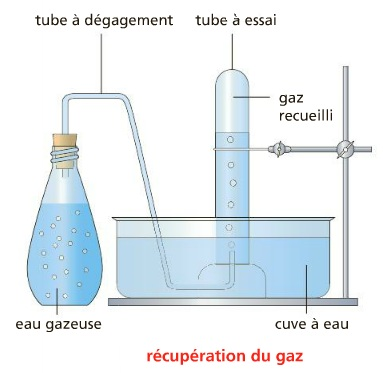
\includegraphics[scale=0.4]{recueilgaz}
		\end{column}

	
\end{columns}.
\end{mybilan}
%\end{frame}
%
%\section{Reconnaître le dioxyde de carbone}
%
%\begin{frame}
%	\begin{myact}{4 page 127}
	\begin{enumerate}
		\item Le gaz prélevé dans la seringue a été extrait d'eau pétillante par déplacement d'eau.\pause
		\item Au début de l'expérience, la solution d'eau de chaux est incolore et transparente.\pause
		\item Après y avoir fait barboter le gaz l'eau de chaux s'est troublée.\pause
		\item Un précipité blanc s'est formé lors de cette expérience, donc le gaz dissous dans l'eau pétillante est du dioxyde de carbone.
	\end{enumerate}
\end{myact}
%\end{frame}
%
%
%\begin{frame}
%	\begin{mybilan}
	\begin{itemize}
		\item La masse d'un corps est \kw{proportionnelle} à son volume; \pause
		\item Le coefficient de proportionnalité est la \kw{masse volumique} (notée $\rho$);\pause
		\item \kw{Un litre d'eau} a une masse de \kw{1 kilogramme};\pause
		\item Une substance est \kw{plus dense} qu'une autre si, pour un même volume, sa masse est supérieure.		
	\end{itemize}
\end{mybilan}
%\end{frame}

\end{document}